% Options for packages loaded elsewhere
\PassOptionsToPackage{unicode}{hyperref}
\PassOptionsToPackage{hyphens}{url}
%
\documentclass[
]{article}
\usepackage{amsmath,amssymb}
\usepackage{lmodern}
\usepackage{ifxetex,ifluatex}
\ifnum 0\ifxetex 1\fi\ifluatex 1\fi=0 % if pdftex
  \usepackage[T1]{fontenc}
  \usepackage[utf8]{inputenc}
  \usepackage{textcomp} % provide euro and other symbols
\else % if luatex or xetex
  \usepackage{unicode-math}
  \defaultfontfeatures{Scale=MatchLowercase}
  \defaultfontfeatures[\rmfamily]{Ligatures=TeX,Scale=1}
\fi
% Use upquote if available, for straight quotes in verbatim environments
\IfFileExists{upquote.sty}{\usepackage{upquote}}{}
\IfFileExists{microtype.sty}{% use microtype if available
  \usepackage[]{microtype}
  \UseMicrotypeSet[protrusion]{basicmath} % disable protrusion for tt fonts
}{}
\makeatletter
\@ifundefined{KOMAClassName}{% if non-KOMA class
  \IfFileExists{parskip.sty}{%
    \usepackage{parskip}
  }{% else
    \setlength{\parindent}{0pt}
    \setlength{\parskip}{6pt plus 2pt minus 1pt}}
}{% if KOMA class
  \KOMAoptions{parskip=half}}
\makeatother
\usepackage{xcolor}
\IfFileExists{xurl.sty}{\usepackage{xurl}}{} % add URL line breaks if available
\IfFileExists{bookmark.sty}{\usepackage{bookmark}}{\usepackage{hyperref}}
\hypersetup{
  pdftitle={Assignment\_2\_6659\_tianni2},
  pdfauthor={Tian Ni},
  hidelinks,
  pdfcreator={LaTeX via pandoc}}
\urlstyle{same} % disable monospaced font for URLs
\usepackage[margin=1in]{geometry}
\usepackage{color}
\usepackage{fancyvrb}
\newcommand{\VerbBar}{|}
\newcommand{\VERB}{\Verb[commandchars=\\\{\}]}
\DefineVerbatimEnvironment{Highlighting}{Verbatim}{commandchars=\\\{\}}
% Add ',fontsize=\small' for more characters per line
\usepackage{framed}
\definecolor{shadecolor}{RGB}{248,248,248}
\newenvironment{Shaded}{\begin{snugshade}}{\end{snugshade}}
\newcommand{\AlertTok}[1]{\textcolor[rgb]{0.94,0.16,0.16}{#1}}
\newcommand{\AnnotationTok}[1]{\textcolor[rgb]{0.56,0.35,0.01}{\textbf{\textit{#1}}}}
\newcommand{\AttributeTok}[1]{\textcolor[rgb]{0.77,0.63,0.00}{#1}}
\newcommand{\BaseNTok}[1]{\textcolor[rgb]{0.00,0.00,0.81}{#1}}
\newcommand{\BuiltInTok}[1]{#1}
\newcommand{\CharTok}[1]{\textcolor[rgb]{0.31,0.60,0.02}{#1}}
\newcommand{\CommentTok}[1]{\textcolor[rgb]{0.56,0.35,0.01}{\textit{#1}}}
\newcommand{\CommentVarTok}[1]{\textcolor[rgb]{0.56,0.35,0.01}{\textbf{\textit{#1}}}}
\newcommand{\ConstantTok}[1]{\textcolor[rgb]{0.00,0.00,0.00}{#1}}
\newcommand{\ControlFlowTok}[1]{\textcolor[rgb]{0.13,0.29,0.53}{\textbf{#1}}}
\newcommand{\DataTypeTok}[1]{\textcolor[rgb]{0.13,0.29,0.53}{#1}}
\newcommand{\DecValTok}[1]{\textcolor[rgb]{0.00,0.00,0.81}{#1}}
\newcommand{\DocumentationTok}[1]{\textcolor[rgb]{0.56,0.35,0.01}{\textbf{\textit{#1}}}}
\newcommand{\ErrorTok}[1]{\textcolor[rgb]{0.64,0.00,0.00}{\textbf{#1}}}
\newcommand{\ExtensionTok}[1]{#1}
\newcommand{\FloatTok}[1]{\textcolor[rgb]{0.00,0.00,0.81}{#1}}
\newcommand{\FunctionTok}[1]{\textcolor[rgb]{0.00,0.00,0.00}{#1}}
\newcommand{\ImportTok}[1]{#1}
\newcommand{\InformationTok}[1]{\textcolor[rgb]{0.56,0.35,0.01}{\textbf{\textit{#1}}}}
\newcommand{\KeywordTok}[1]{\textcolor[rgb]{0.13,0.29,0.53}{\textbf{#1}}}
\newcommand{\NormalTok}[1]{#1}
\newcommand{\OperatorTok}[1]{\textcolor[rgb]{0.81,0.36,0.00}{\textbf{#1}}}
\newcommand{\OtherTok}[1]{\textcolor[rgb]{0.56,0.35,0.01}{#1}}
\newcommand{\PreprocessorTok}[1]{\textcolor[rgb]{0.56,0.35,0.01}{\textit{#1}}}
\newcommand{\RegionMarkerTok}[1]{#1}
\newcommand{\SpecialCharTok}[1]{\textcolor[rgb]{0.00,0.00,0.00}{#1}}
\newcommand{\SpecialStringTok}[1]{\textcolor[rgb]{0.31,0.60,0.02}{#1}}
\newcommand{\StringTok}[1]{\textcolor[rgb]{0.31,0.60,0.02}{#1}}
\newcommand{\VariableTok}[1]{\textcolor[rgb]{0.00,0.00,0.00}{#1}}
\newcommand{\VerbatimStringTok}[1]{\textcolor[rgb]{0.31,0.60,0.02}{#1}}
\newcommand{\WarningTok}[1]{\textcolor[rgb]{0.56,0.35,0.01}{\textbf{\textit{#1}}}}
\usepackage{graphicx}
\makeatletter
\def\maxwidth{\ifdim\Gin@nat@width>\linewidth\linewidth\else\Gin@nat@width\fi}
\def\maxheight{\ifdim\Gin@nat@height>\textheight\textheight\else\Gin@nat@height\fi}
\makeatother
% Scale images if necessary, so that they will not overflow the page
% margins by default, and it is still possible to overwrite the defaults
% using explicit options in \includegraphics[width, height, ...]{}
\setkeys{Gin}{width=\maxwidth,height=\maxheight,keepaspectratio}
% Set default figure placement to htbp
\makeatletter
\def\fps@figure{htbp}
\makeatother
\setlength{\emergencystretch}{3em} % prevent overfull lines
\providecommand{\tightlist}{%
  \setlength{\itemsep}{0pt}\setlength{\parskip}{0pt}}
\setcounter{secnumdepth}{-\maxdimen} % remove section numbering
\ifluatex
  \usepackage{selnolig}  % disable illegal ligatures
\fi

\title{Assignment\_2\_6659\_tianni2}
\author{Tian Ni}
\date{9/23/2021}

\begin{document}
\maketitle

\hypertarget{part-i.}{%
\subsection{Part I.}\label{part-i.}}

First load the transformed Boston Housing Data

\begin{Shaded}
\begin{Highlighting}[]
\NormalTok{myData}\OtherTok{=}\FunctionTok{read.csv}\NormalTok{(}\StringTok{"Coding2\_myData.csv"}\NormalTok{,}\AttributeTok{header =} \ConstantTok{TRUE}\NormalTok{)}
\NormalTok{X}\OtherTok{=}\FunctionTok{as.matrix}\NormalTok{(myData[,}\SpecialCharTok{{-}}\DecValTok{14}\NormalTok{])}
\NormalTok{y}\OtherTok{=}\NormalTok{myData}\SpecialCharTok{$}\NormalTok{Y}
\FunctionTok{dim}\NormalTok{(X)}
\end{Highlighting}
\end{Shaded}

\begin{verbatim}
## [1] 506  13
\end{verbatim}

Then we construct the one\_var\_lasso function which could be used to
solve the Lasso estimate for \(\beta_{j}\) given other coefficients
fixed

\begin{Shaded}
\begin{Highlighting}[]
\NormalTok{one\_var\_lasso}\OtherTok{=}\ControlFlowTok{function}\NormalTok{(r,x,lam)\{}
\NormalTok{  xx}\OtherTok{=}\FunctionTok{sum}\NormalTok{(x}\SpecialCharTok{\^{}}\DecValTok{2}\NormalTok{)}
\NormalTok{  xr}\OtherTok{=}\FunctionTok{sum}\NormalTok{(r}\SpecialCharTok{*}\NormalTok{x)}
\NormalTok{  b}\OtherTok{=}\NormalTok{(}\FunctionTok{abs}\NormalTok{(xr)}\SpecialCharTok{{-}}\NormalTok{lam}\SpecialCharTok{/}\DecValTok{2}\NormalTok{)}\SpecialCharTok{/}\NormalTok{xx}
\NormalTok{  b}\OtherTok{=}\FunctionTok{sign}\NormalTok{(xr) }\SpecialCharTok{*} \FunctionTok{ifelse}\NormalTok{(b}\SpecialCharTok{\textgreater{}}\DecValTok{0}\NormalTok{, b, }\DecValTok{0}\NormalTok{)}
  \FunctionTok{return}\NormalTok{(b)}
\NormalTok{\}}
\end{Highlighting}
\end{Shaded}

Then we construct our MyLasso function which could implement CD and
output estimated Lasso coefficients

\begin{Shaded}
\begin{Highlighting}[]
\NormalTok{MyLasso}\OtherTok{=}\ControlFlowTok{function}\NormalTok{(X, y, lam.seq, }\AttributeTok{maxit=}\DecValTok{100}\NormalTok{)\{}
  \CommentTok{\# X: n{-}by{-}p design matrix without the intercept}
  \CommentTok{\# y: n{-}by{-}1 response vector}
  \CommentTok{\# lam.seq: sequence of lambda values (arranged from large to small)}
  \CommentTok{\# maxit: number of updates for each lambda}
  \CommentTok{\# Center/Scale X}
  \CommentTok{\# Center y}
  
\NormalTok{  n}\OtherTok{=}\FunctionTok{length}\NormalTok{(y)}
\NormalTok{  p}\OtherTok{=}\FunctionTok{dim}\NormalTok{(X)[}\DecValTok{2}\NormalTok{]}
\NormalTok{  nlam}\OtherTok{=}\FunctionTok{length}\NormalTok{(lam.seq)}
  
  \CommentTok{\# Now we scale and center X and y}
\NormalTok{  y.mean}\OtherTok{=}\FunctionTok{mean}\NormalTok{(y)}
\NormalTok{  X.mean}\OtherTok{=}\FunctionTok{apply}\NormalTok{(X,}\DecValTok{2}\NormalTok{,mean)}
\NormalTok{  X.sd}\OtherTok{=}\FunctionTok{apply}\NormalTok{(X, }\DecValTok{2}\NormalTok{, sd)}
\NormalTok{  Xs}\OtherTok{=}\FunctionTok{scale}\NormalTok{(X,}\AttributeTok{center =}\NormalTok{ X.mean, }\AttributeTok{scale =}\NormalTok{ X.sd)}
  
  \CommentTok{\# Initialize coef vector b and residual vector r}
\NormalTok{  b}\OtherTok{=}\FunctionTok{rep}\NormalTok{(}\DecValTok{0}\NormalTok{,p)}
\NormalTok{  r}\OtherTok{=}\NormalTok{y}
\NormalTok{  B}\OtherTok{=}\FunctionTok{matrix}\NormalTok{(}\AttributeTok{nrow =}\NormalTok{ nlam,}\AttributeTok{ncol =}\NormalTok{ p}\SpecialCharTok{+}\DecValTok{1}\NormalTok{)}
  
  \CommentTok{\# Triple nested loop}
  \ControlFlowTok{for}\NormalTok{ (m }\ControlFlowTok{in} \DecValTok{1}\SpecialCharTok{:}\NormalTok{nlam) \{}
\NormalTok{    lam}\OtherTok{=}\DecValTok{2}\SpecialCharTok{*}\NormalTok{n}\SpecialCharTok{*}\NormalTok{lam.seq[m]}
    \ControlFlowTok{for}\NormalTok{(step }\ControlFlowTok{in} \DecValTok{1}\SpecialCharTok{:}\NormalTok{ maxit)\{}
      \ControlFlowTok{for}\NormalTok{(j }\ControlFlowTok{in} \DecValTok{1}\SpecialCharTok{:}\NormalTok{p)\{}
\NormalTok{        r}\OtherTok{=}\NormalTok{r}\SpecialCharTok{+}\NormalTok{(Xs[,j]}\SpecialCharTok{*}\NormalTok{b[j])}
\NormalTok{        b[j]}\OtherTok{=}\FunctionTok{one\_var\_lasso}\NormalTok{(r,Xs[,j],lam)}
\NormalTok{        r}\OtherTok{=}\NormalTok{r}\SpecialCharTok{{-}}\NormalTok{(Xs[,j]}\SpecialCharTok{*}\NormalTok{b[j])}
\NormalTok{      \}}
\NormalTok{    \}}
\NormalTok{    B[m,]}\OtherTok{=}\FunctionTok{c}\NormalTok{(}\DecValTok{0}\NormalTok{,b)}
\NormalTok{  \}}
  
  \CommentTok{\# Now we update the intercepts stored in B[,1]}
\NormalTok{  B[,}\DecValTok{1}\NormalTok{]}\OtherTok{=}\NormalTok{y.mean}\SpecialCharTok{{-}}\NormalTok{(X.mean}\SpecialCharTok{/}\NormalTok{X.sd) }\SpecialCharTok{\%*\%} \FunctionTok{t}\NormalTok{(B[,}\DecValTok{2}\SpecialCharTok{:}\NormalTok{(p}\SpecialCharTok{+}\DecValTok{1}\NormalTok{)])}
  
  \CommentTok{\# Now we scale back the coefficients}
\NormalTok{  B[,}\DecValTok{2}\SpecialCharTok{:}\NormalTok{(p}\SpecialCharTok{+}\DecValTok{1}\NormalTok{)]}\OtherTok{=}\FunctionTok{scale}\NormalTok{(B[,}\DecValTok{2}\SpecialCharTok{:}\NormalTok{(p}\SpecialCharTok{+}\DecValTok{1}\NormalTok{)],}\AttributeTok{center =} \ConstantTok{FALSE}\NormalTok{,}\AttributeTok{scale=}\NormalTok{X.sd)}
  
  \FunctionTok{return}\NormalTok{(}\FunctionTok{t}\NormalTok{(B))}
\NormalTok{\}}
\end{Highlighting}
\end{Shaded}

Now we test our algorithm

\begin{Shaded}
\begin{Highlighting}[]
\NormalTok{lam.seq}\OtherTok{=}\FunctionTok{exp}\NormalTok{(}\FunctionTok{seq}\NormalTok{(}\SpecialCharTok{{-}}\DecValTok{1}\NormalTok{,}\SpecialCharTok{{-}}\DecValTok{8}\NormalTok{,}\AttributeTok{length.out=}\DecValTok{80}\NormalTok{))}
\NormalTok{myout}\OtherTok{=}\FunctionTok{MyLasso}\NormalTok{(X,y,lam.seq, }\AttributeTok{maxit =} \DecValTok{50}\NormalTok{)}
\FunctionTok{rownames}\NormalTok{(myout)}\OtherTok{=}\FunctionTok{c}\NormalTok{(}\StringTok{"Intercept"}\NormalTok{,}\FunctionTok{colnames}\NormalTok{(X))}
\FunctionTok{dim}\NormalTok{(myout)}
\end{Highlighting}
\end{Shaded}

\begin{verbatim}
## [1] 14 80
\end{verbatim}

Now produce the path plot for the 12 non-intercept coefficients with the
x-coordinate to be the lambda values in log-scale.

\begin{Shaded}
\begin{Highlighting}[]
\NormalTok{x.index }\OtherTok{=} \FunctionTok{log}\NormalTok{(lam.seq)}
\NormalTok{beta}\OtherTok{=}\NormalTok{myout[}\SpecialCharTok{{-}}\DecValTok{1}\NormalTok{,]}
\FunctionTok{matplot}\NormalTok{(x.index, }\FunctionTok{t}\NormalTok{(beta), }\AttributeTok{xlim=}\FunctionTok{c}\NormalTok{(}\FunctionTok{min}\NormalTok{(x.index),}\FunctionTok{max}\NormalTok{(x.index)),}
        \AttributeTok{lty =} \DecValTok{1}\NormalTok{, }\AttributeTok{xlab=}\StringTok{"Log Lambda"}\NormalTok{, }\AttributeTok{ylab=}\StringTok{"Coefficients"}\NormalTok{, }\AttributeTok{type=}\StringTok{"l"}\NormalTok{, }\AttributeTok{lwd=}\DecValTok{1}\NormalTok{)}

\CommentTok{\# Add variable names to each path}
\NormalTok{var.names}\OtherTok{=}\FunctionTok{colnames}\NormalTok{(X)}
\NormalTok{nvar}\OtherTok{=}\FunctionTok{length}\NormalTok{(var.names)}
\NormalTok{xpos}\OtherTok{=}\FunctionTok{rep}\NormalTok{(}\FunctionTok{min}\NormalTok{(x.index),nvar)}
\NormalTok{ypos}\OtherTok{=}\NormalTok{beta[,}\FunctionTok{ncol}\NormalTok{(beta)]}
\FunctionTok{text}\NormalTok{(xpos,ypos,var.names,}\AttributeTok{cex=}\FloatTok{0.5}\NormalTok{,}\AttributeTok{pos=}\DecValTok{2}\NormalTok{)}
\end{Highlighting}
\end{Shaded}

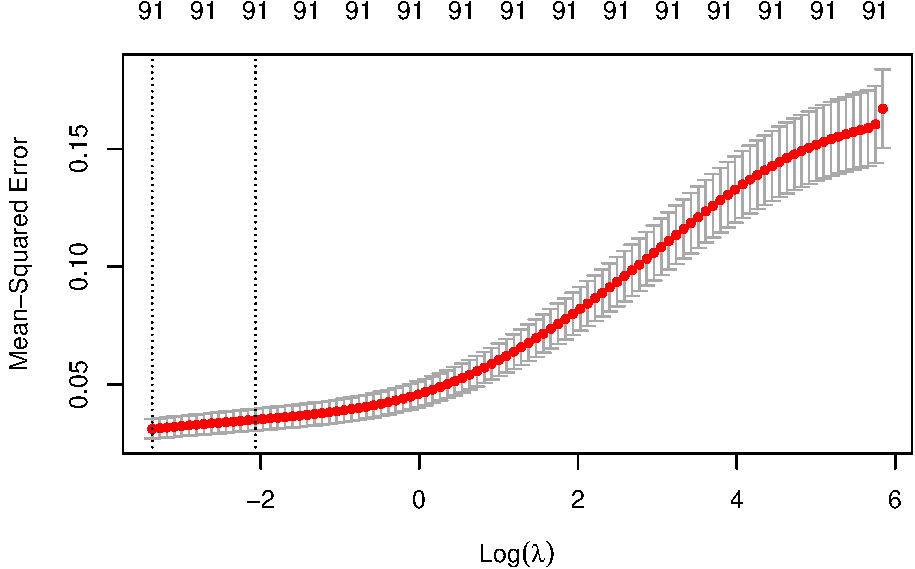
\includegraphics{Assignment_2_6659_tianni2_files/figure-latex/unnamed-chunk-5-1.pdf}

Check accuracy

\begin{Shaded}
\begin{Highlighting}[]
\FunctionTok{library}\NormalTok{(glmnet)}
\end{Highlighting}
\end{Shaded}

\begin{verbatim}
## 载入需要的程辑包:Matrix
\end{verbatim}

\begin{verbatim}
## Loaded glmnet 4.1-2
\end{verbatim}

\begin{Shaded}
\begin{Highlighting}[]
\NormalTok{lasso.fit}\OtherTok{=}\FunctionTok{glmnet}\NormalTok{(X,y,}\AttributeTok{alpha=}\DecValTok{1}\NormalTok{,}\AttributeTok{lambda=}\NormalTok{lam.seq)}
\FunctionTok{max}\NormalTok{(}\FunctionTok{abs}\NormalTok{(}\FunctionTok{coef}\NormalTok{(lasso.fit)}\SpecialCharTok{{-}}\NormalTok{myout))}
\end{Highlighting}
\end{Shaded}

\begin{verbatim}
## [1] 0.004597206
\end{verbatim}

\begin{Shaded}
\begin{Highlighting}[]
\FunctionTok{plot}\NormalTok{(lasso.fit,}\AttributeTok{xvar=}\StringTok{"lambda"}\NormalTok{)}
\end{Highlighting}
\end{Shaded}

\includegraphics{Assignment_2_6659_tianni2_files/figure-latex/unnamed-chunk-6-1.pdf}

\begin{Shaded}
\begin{Highlighting}[]
\FunctionTok{detach}\NormalTok{(}\StringTok{"package:glmnet"}\NormalTok{)}
\end{Highlighting}
\end{Shaded}


\end{document}
